Pingo ist eine Software-Lösung, die bereits seit dem Jahr 2011 an der Universität Paderborn entwickelt wird. Der Name ist ebenfalls ein Akronym und steht für „\textbf{P}eer \textbf{In}struction for Very Large \textbf{G}r\textbf{o}ups“. Im Gegensatz zu StuReSy ist Pingo bereits weiter verbreitet und wird an vielen deutschen Hochschulen eingesetzt – im September 2018 gab es 22.000 angemeldete Nutzer (vgl. \cite{web:pingo_zukunft}). Dahinter stand außerdem ein ganzes Team akademischer Mitarbeiter (vgl. \cite{web:pingo_team}). Seit 2019 wird Pingo von der universitätsnahen Coactum GmbH betrieben und weiterentwickelt (vgl. \cite{web:pingo_coactum}). Das Projekt ist damit deutlich professioneller ausgerichtet als StuReSy.

Im Gegensatz zu StuReSy ist Pingo eine reine Web-Applikation, die öffentlich unter \url{http://trypingo.com/} auffindbar ist und kostenlos genutzt werden kann. Sowohl Administratoren als auch Teilnehmer können alle Arbeiten im Browser erledigen, ein Software-Download ist nicht notwendig. Für die administrative Nutzung muss jedoch ein Benutzerkonto erstellt werden. Einzelne Sitzungen werden durch numerische IDs im Namensraum eines Pingo-Servers identifiziert.


Eine Direktverbindung zwischen Umfrage-Teilnehmern wird nicht unterstützt, stattdessen wird eine Pingo-Server vorausgesetzt. Der Betreiber stellt einen öffentlichen Pingo-Server kostenlos zur Verfügung. Pingo steht aber unter einer Open-Source-Lizenz, so dass Nutzer auch eine eigene Instanz betreiben können. Pingo ist in der Programmiersprache Ruby und mithilfe des Web-Frameworks „Ruby on Rails“ implementiert (vgl. \cite{web:pingo_github}). Entsprechend dazu muss ein potenzieller Server auch über einen Ruby-Interpreter und über eine NoSQL-Datenbank verfügen, um Pingo ausführen zu können.

In ihren Kernfunktionen sind sich Pingo und StuReSy sehr ähnlich. Trotzdem fehlt eine kritische Funktionen für den Einsatz in der Programmierlehre:

Fragen innerhalb der Pingo-Plattform können überhaupt nicht formatiert werden. Damit können selbst simple Formatierungen wie Fettschreibungen, Unterstreichungen oder Zeilenumbrüche nicht verwendet werden (erkennbar in Abbildung \ref{abb:pingo_frage}). Dementsprechend ist auch die übersichtliche Darstellung von Quelltext unmöglich und Pingo für den Einsatz in der Programmierlehre ungeeignet.


\begin{figure}[H]
    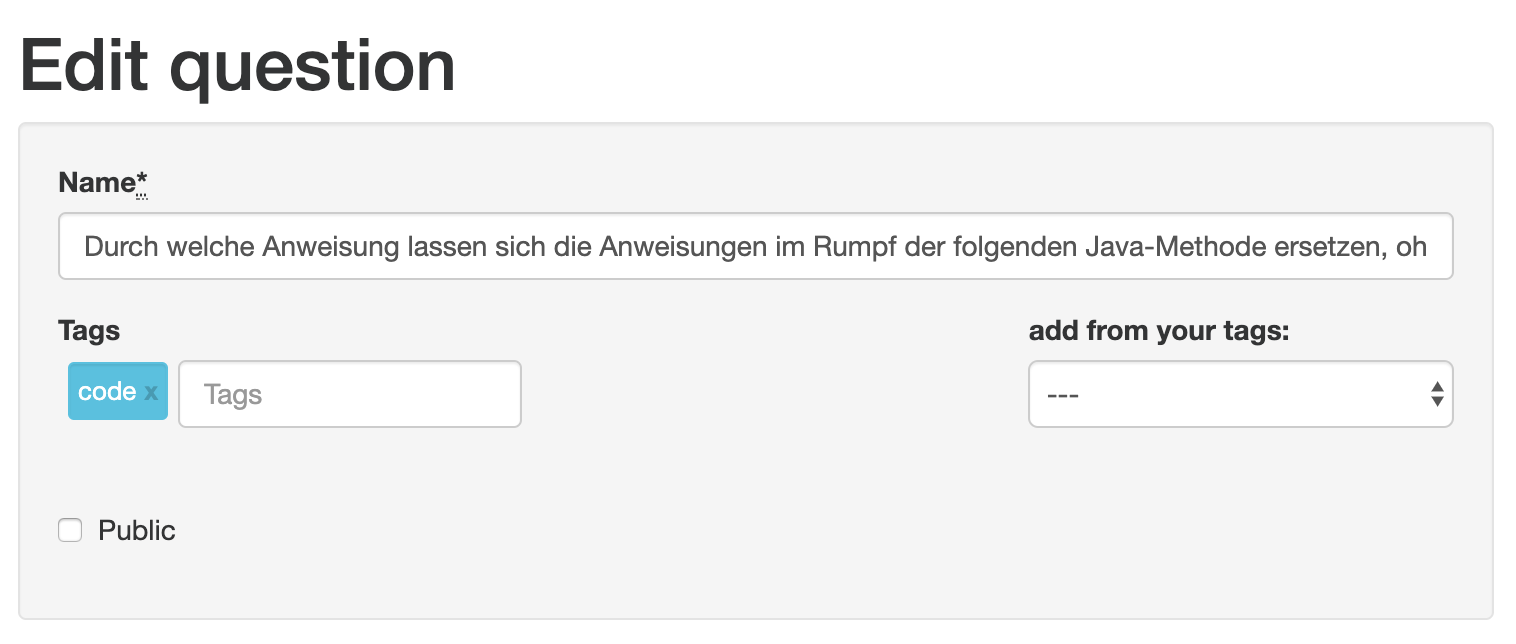
\includegraphics[width=12cm]{chapter/bewertung/bilder/pingo_editor.png}
    \centering
    \caption[Fragen-Editor in Pingo ohne Formatierungsmöglichkeiten]{Der Fragen-Editor von Pingo verfügt über keine Formatierungsmöglichkeiten.}
    \label{abb:pingo_editor}
\end{figure}


\begin{figure}[H]
    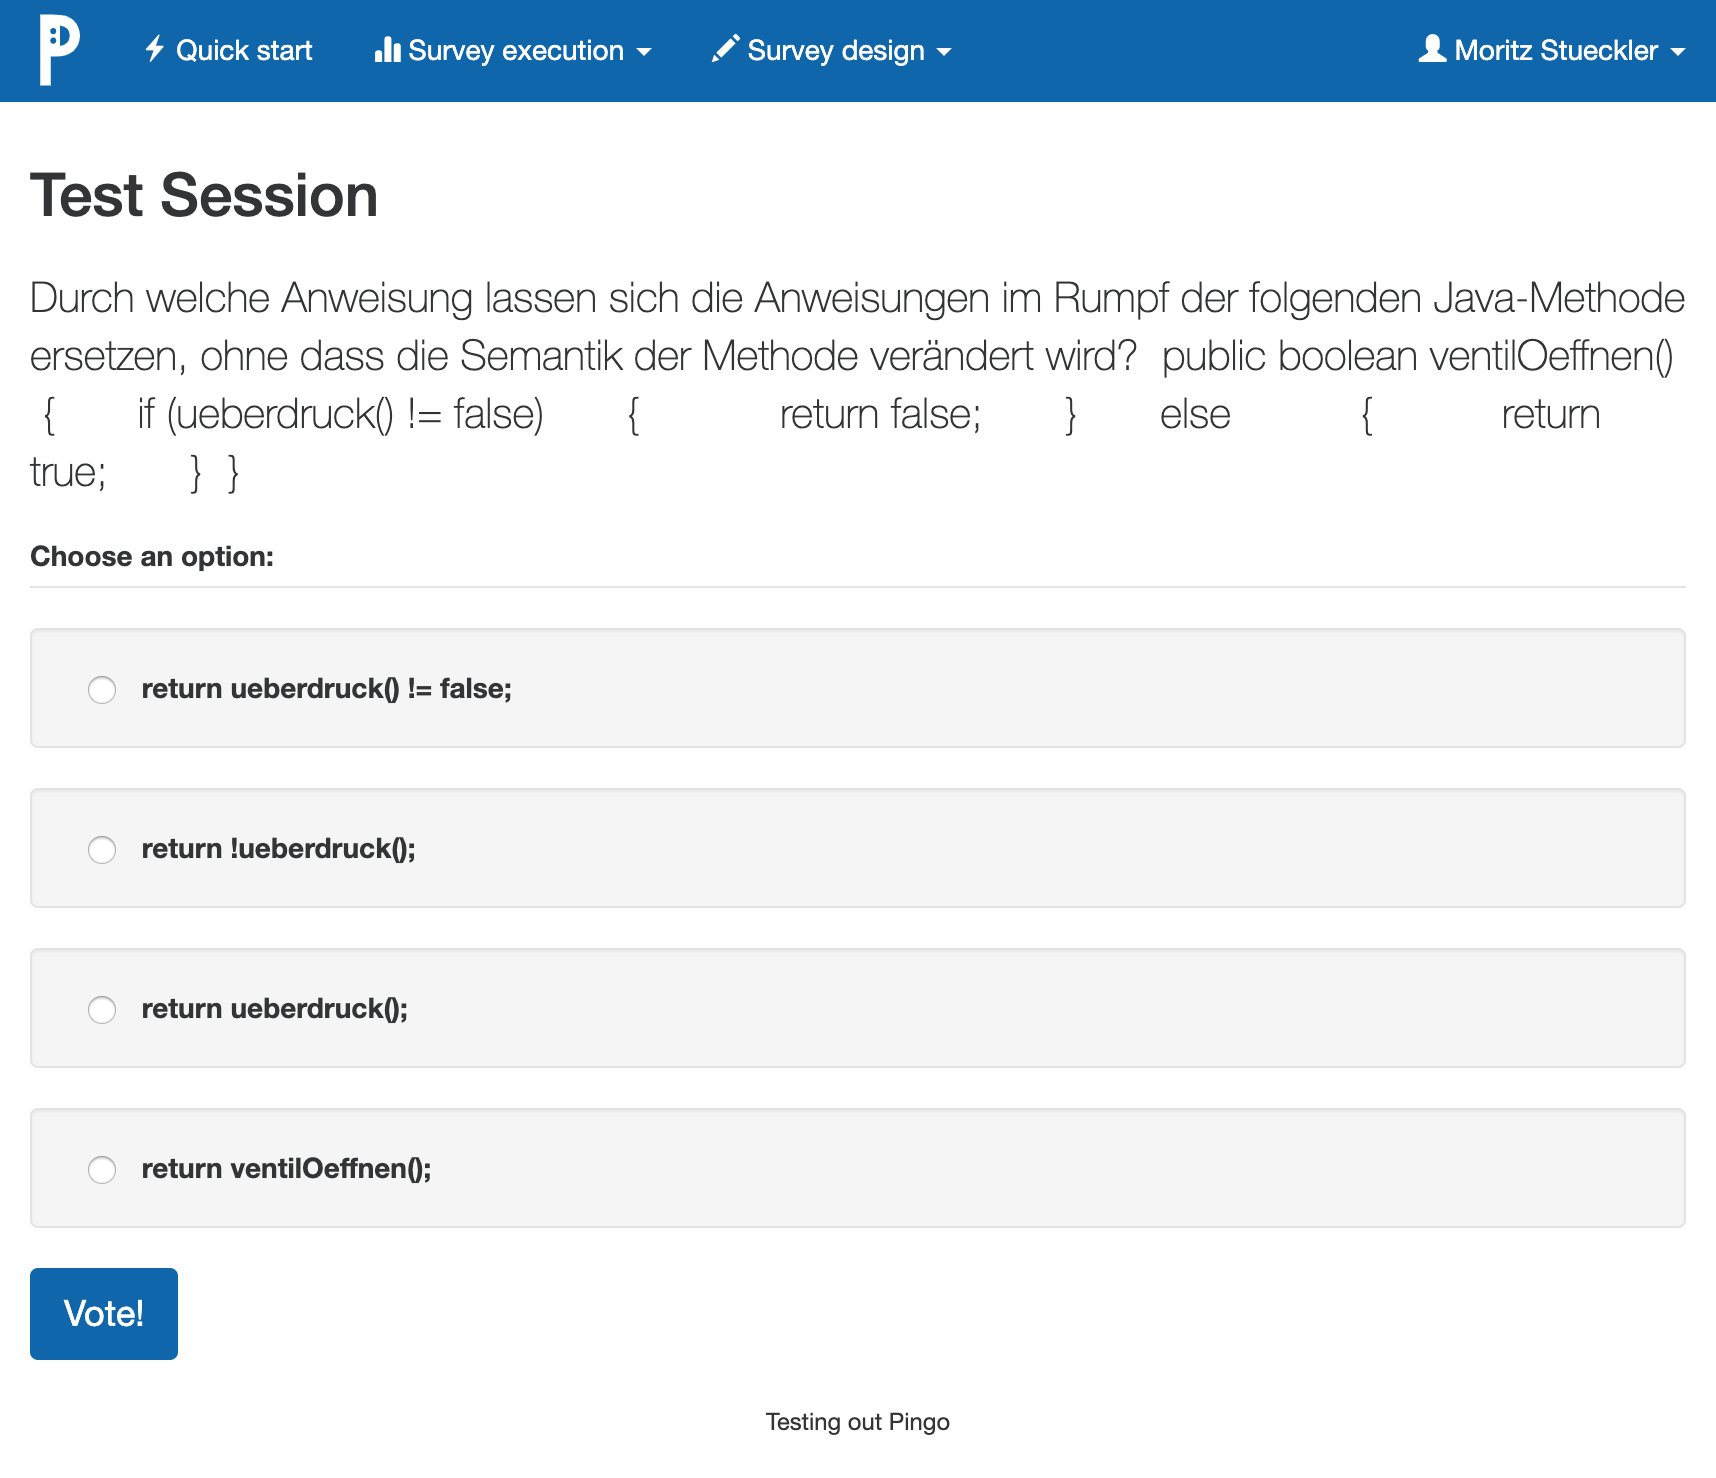
\includegraphics[width=12cm]{chapter/bewertung/bilder/pingo_problem1.png}
    \centering
    \caption[Darstellung von Quelltexten in Pingo]{Eine ordentliche Darstellung von Quelltexten ohne Textformatierungen ist nicht möglich.}
    \label{abb:pingo_frage}
\end{figure}
